En este laboratorio se busca  determinar la concentración tóxica de nanodiamantes fluorescentes mediante una técnica de caraterización en vitro.

\textbf{\textcolor{azul50}{Formalismo}}

Dado que las nanopartículas pueden ser producidas con distintos tamaños, formas y conservan la capacidad de ser funcionalizados utilizando un amplio abanico de ligandos entre
los cuales se encuentran los anticuerpos, polímeros,
fármacos y material genético, se ha despertado un gran interés en
el campo de la biomedicina. 

Al ser muy estables y poseer una alta
biocompatibilidad, los nanodiamantes permiten colocar elementos
químicos sobre su superficie produciendo un sistema
completamente funcional (nanodiamante-elemento), por lo cual recientes investigaciones demostraron que los nanodiamantes pueden utilizarse para transportar el fármaco quimioterapéutico hasta el tumor cancerígeno, este innovador tratamiento presenta una gran efectividad para mermar el cáncer y una reducción de los efectos secundarios perjudiciales por su biocompatibilidad.

\begin{figure}
    %\centering
    %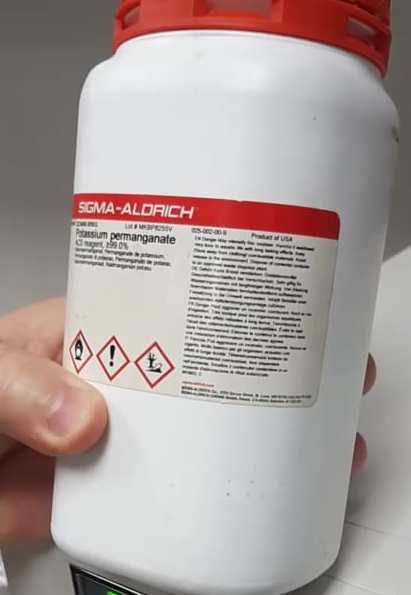
\includegraphics[width=0.3\textwidth]{Tarea1/muestras.png}
    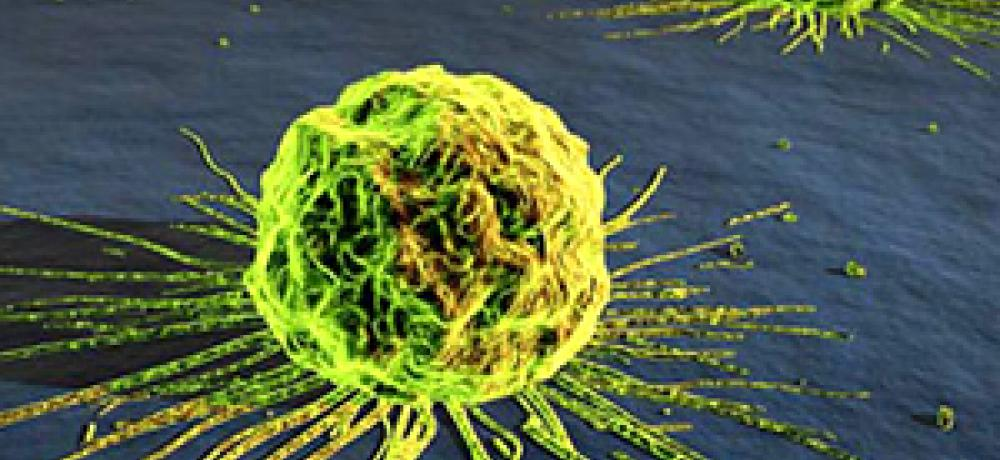
\includegraphics[width=0.49\textwidth]{Tarea5/nano.png}
    \caption{\textbf{Nanodiamantes presentados en la revista de Science Translational Medicine.}}
    \label{nano}
\end{figure}

Actualmente ya es posible por los científicos crear una combinación de fármaco y nanodiamante que puede ser inyectado en los tumores, consiguiendo así una mayor retención del químico en el interior del tumor y por ende un aumento de la eficacia del tratamiento sin afectar a los tejidos cercanos y de esta forma reducir los efectos tóxicos derivados de la quimioterapia. Esto presenta un gran avance en los tratamientos actuales ya que los tumores de manera general son difíciles de tratar debido a que los fármacos de la quimioterapia inyectados son incapaces de penetrar en ciertas partes del sistema de protección de vasos sanguíneos (ejemplo de este es el que rodea el cerebro). 



Este hallazgo demuestra que la colaboración entre bioingeniería y medicina es fundamental para desarrollar un futuro tratamiento menos nocivo y más contundente contra la enfermedad.

\textbf{Conteo de celulas en una cámara de Neubauer.}

La cámara de Neubauer es un instrumento utilizado en medicina y biología para realizar el recuento de esporas y células en un medio líquido, que puede ser; un cultivo celular, sangre, orina, líquido cefalorraquídeo, líquido sinovial, etc.

La misma tradicionalmente está adaptada al microscopio (Fig. \ref{microscopio}), ella tiene forma de un portaobjetos que tiene dos zonas ligeramente deprimidas en cuyo fondo se ha marcado con la ayuda de un diamante una cuadrícula de dimensiones conocidas. Se cubre la cámara con un cubreobjetos que se adhiere por simple tensión superficial (en especial una vez que se haya añadido la muestra líquida).

Luego se introduce por capilaridad entre la cámara y el cubre, el líquido con las células a contar, generalmente tras una dilución previa; la cámara tiene dos zonas lo que permite hacer dos recuentos simultáneamente. Se observa la retícula al microscopio con el aumento adecuado y se cuentan las células.

A partir del número de células contadas, conociendo el volumen de líquido que admite el campo de la retícula, se cálcula la concentración de células en la muestra líquida aplicada. El cálculo de la concentración de células se puede expresar así:
\begin{equation}
    \label{concentracion}
    C_T = \dfrac{C_o}{(A)\cdot (h) }\cdot \delta
\end{equation}
donde $C_T$ es la concentracion por mililitros cúbicos, $C_o$ conteo de partículas, $A$ es el área de la camara de conteo, $h$ profundidad de la cámara y $\delta$ es la dilución.

En la retícula central, la cámara de Neubauer tiene un cuadrado primario que contiene nueve cuadrados secundarios, cada uno de ellos dividido a su vez en 16 cuadrados terciarios. El cuadrado secundario central contiene no 16, sino 25 cuadrados, cada uno de ellos dividido a su vez en 16 cuadrados cuaternarios. En los bordes de este cuadrado central se cuentan los hematíes, utilizando sólo los cuadrados de los bordes del terciario central y uno de los centrales. En los secundarios de los bordes superiores e inferiores de la cámara se hace el recuento leucocitario.


\textbf{Estudios de Toxicidad de nanodiamentes con el espectrofotómetro.}

Otro problema muy común en el área de producción es que cuando se diseña y sintetiza un material nuevo, con el objetivo de estudiar su comportamiento para alguna aplicación futura, como parte del proceso de caracterización se precisa estudiar su toxicidad para su posterior producción, manipulación y comercialización ya que pueden provocar daño a nivel fisiológico, esto hace que los estudios en vitro sean un primer acercamiento práctico y rápido.

\textbf{\textcolor{azul50}{Procedimiento Experimental}}

Se análizará la capacidad de toxicidad que posee las nanopartículas sobre células vivas para esto se hizo uso de diferentes sustancias, entre ellas:

\begin{itemize}
    \item \textbf{\textcolor{morado}{RPMI:}} El medio Roswell Park Memorial Institute (en inglés, Roswell Park Memorial Institute medium),el mismo es usado para cultivos celulares. Tradicionalmente, es usado para el cultivo de células humanas o de tejidos aislados como el caso de las arterias mamarias humanas.
    \item \textbf{\textcolor{morado}{T-47D:}} es una línea celular de cáncer de seno humano comúnmente utilizada en la investigación biomédica que involucra la expresión hormonal de células cancerosas.
    %\item \textbf{\textcolor{morado}{MDA:}} es una de las líneas celulares es una de las más utilizadas para el estudio experimental in vitro del cáncer de mama hormono-independiente. Estás células presentan un crecimiento extraordinariamente rápido en medios de cultivo poco enriquecidos. Se utilizan en estudios bioquímicos y genéticos que han contribuido enormemente a la investigación del cáncer de mama y al desarrollo de fármacos para ayudar a combatirlo.
    \item \textbf{\textcolor{morado}{Azul de metileno:}} 
    se utiliza como colorante en las tinciones para la observación en el microscopio, y para teñir resultados en los laboratorios.
    \item \textbf{\textcolor{morado}{Nanopartículas fluorescentes $900174-5ML$:}} se emplean en diversos métodos de imagen y seguimiento para estudiar cómo las células madre se incorporan y regeneran, al implacar está técnica se implantan en las células madre diminutos diamantes y de esta forma las partículas fluorescentes permiten un seguimiento in vivo de las células.
    \item \textbf{\textcolor{morado}{DmSO:}} Dimetil Sulfóxido, este líquido orgánico incoloro de fórmula química $CH_3SOCH_3$ que contiene sulfóxido, usado como disolvente orgánico industrial a partir de 1940, es utilizado como criopreservante y como un medicamento, posee la propiedad de atravesar rápidamente la epidermis y las membranas celulares, tambien es un disolvente aprótico y altamente polar, por ello, es miscible tanto con el agua como con disolventes orgánicos como alcoholes, cetonas etc. 
\end{itemize}

Primeramente se ralizará el conteo de células para T-47D, para esto se procedió:\\[-1cm]
\begin{itemize}
    \item Se aplicará azúl de tripano en muestras de $T-47D$.
    \item Colocamos las células teñidas en la cámara de Neubauer y realizamos el conteo con el microscopio óptico de la Fig.\ref{microscopio} de las células muertas (coloreadas de azul) y las vivas en los cuadros de control de la cámara.
    \item Se procede al cálculo de las células vivas y muestras por $ml$ haciendo uso de la ec. \ref{concentracion}. 
\end{itemize}

Para valorar la toxicidad de las nanopartículas se procederá con el siguiente experimento:\\[-1cm]
\begin{itemize}
    \item Ya con el valor de $C_T$ obtenido del experimento anterior, se colocan $100\mu l$ del cultivo celular con RPMI en nuestra microplaca.
    \item Se mezclan con los nanodiamantes fluorescentes de forma de que las proporciones sean semejantes a las utilizadas en el procedimiento (B) de la práctica 2 (seccion de obtención de datos).
    \item Se deja repozar hasta el día siguiente, retiramos los nanodiamantes lavando 2 veces con $200~\mu l$ de solución salina y añadimos $100~ \mu l$ de solución RPMI con MTT.
    \item Se deja 30 minutos en incubadora. Retiramos MTT de todas las celdas. Agregamos $50 ~\mu l$ de DmSO en el portamuestras para disolver.
    \item Los resultados de la microplaca se valoraran con el espectrofotómetro de haz monocromático a $570~ nm$.
\end{itemize}

\textbf{\textcolor{azul50}{Análisis de Resultados}}

Al implementar el procedimiento con la camará de Neubauer para una muestra de $T-47D$ se obtuvieron los resultados mostrados en la Fig. \ref{conteo}.
\begin{figure}
    %\centering
    %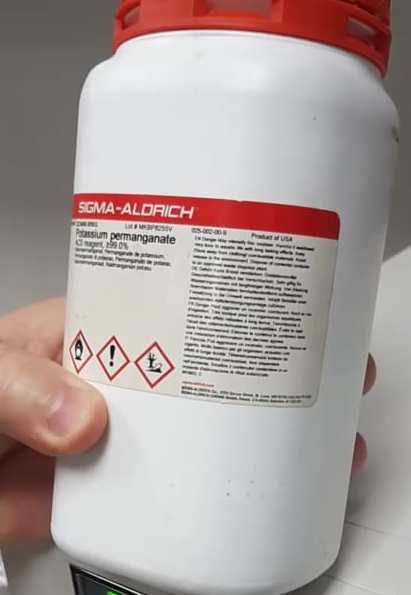
\includegraphics[width=0.3\textwidth]{Tarea1/muestras.png}
    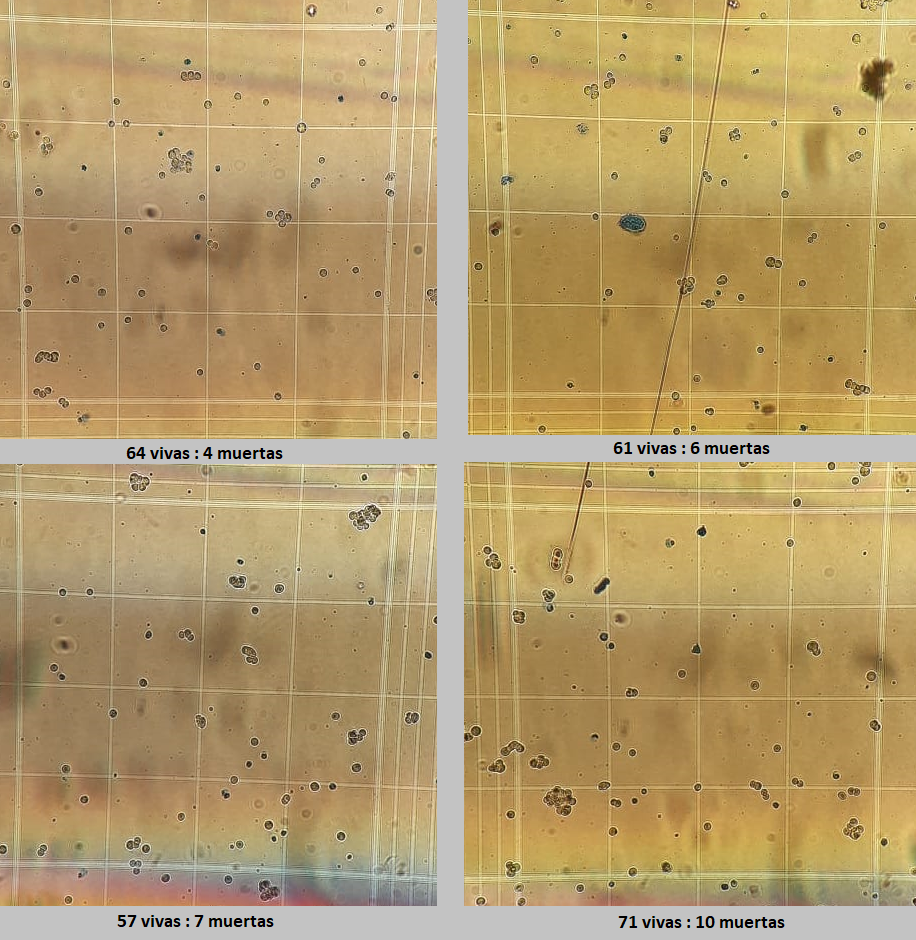
\includegraphics[width=0.39\textwidth]{Tarea5/conteo.png}
    \caption{\textbf{imagenes obtenidas por el microscopio electrónico.}}
    \label{conteo}
\end{figure}
Se puede concluir que entre $6.3\% - 14.3\%$ de las células estaban muertas. Resultado de la implementación de la ec. \ref{concentracion} tenemos que $C_T\approx (15.8 \pm 1.5)\cdot 10^6 ~~cell/ml$, para células vivas. Al obtener y gráficar los resultados reportados por el espectrofotómetro, obtenemos los resultados mostrados en la Fig. \ref{toxicidad}.

El gráfico muestra cambios en la presencia de cristales formados en nuestra muestra, de aquí se puede concluir que si hay efectos de toxicidad visibles como resultado de la presencia de las nanopartículas en nuestra muestra, un análisis de ajuste no fue considerado ya que existe mucha dispersión en los valores obtenidos y existen pocos casos tratados como para considerarlo.
\begin{figure}
    %\centering
    %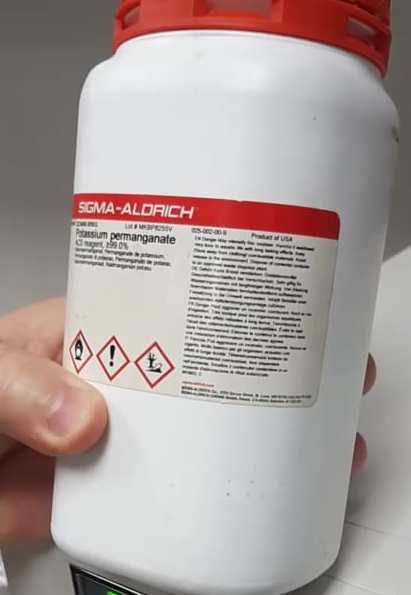
\includegraphics[width=0.3\textwidth]{Tarea1/muestras.png}
    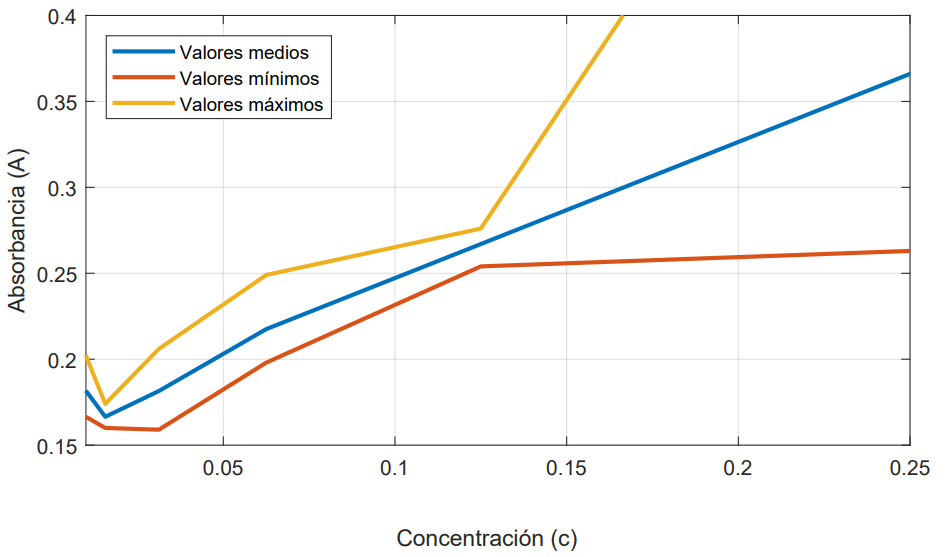
\includegraphics[width=0.49\textwidth]{Tarea5/nano_con_cell.png}
    \caption{\textbf{Procesamiento de los valores de Absorbancia.}}
    \label{toxicidad}
\end{figure}



\textbf{\textcolor{azul50}{Conclusiones}}

El objetivo del laboratorio fue cumplido mediante el conteo utilizando la cámara de Neubauer y al realizar el respectivo análisis de muestras celulares, se comprobó que las nanopartículas si poseen un efecto de toxicidad, no se logró profundizar por la falta de datos, con esto se cumple el objetivo del laboratorio.
